% !TEX root = ../main.tex
\section{已知拓扑下的动力学学习}

\subsection{局部交互表示}

当网络已知时，问题看似只是从 $\mathbf X(t)$ 预测 $\mathbf X(t+1)$，但真正关心的是模型能否形成可复用的局部更新规律。
对许多网络动力学而言，
节点变化都可以理解为两部分共同作用：一部分来自节点自身的状态和内在演化，
另一部分来自邻居传入的交互。
若模型把两者过早压入同一表示，
它可能依靠训练数据中的相关性获得不错的短期预测，
却在节点度数、网络类型或初始条件变化时产生不稳定响应。

SIR 案例把这一问题表现得十分清楚。
感染节点能否康复主要取决于自身状态，易感节点能否感染则取决于感染者邻居的绝对数量。
使用邻居均值时，
模型更容易看到感染邻居的比例，
而非数量；
在不同度数节点上，
相同的比例可能对应完全不同的感染风险。
因此本文使用求和聚合保存交互数量，
并把均值聚合作为对照。

\subsection{融合式基线与双通道表示}

本文的 GraphConv 基线并不是把自身和邻居原始特征直接相加。
其一层更新为
\begin{equation}
\mathbf h_i^{(\ell+1)}=\sigma\!\left(
W_{\mathrm{self}}^{(\ell)}\mathbf h_i^{(\ell)}
+W_{\mathrm{neigh}}^{(\ell)}
\sum_{j\in\mathcal N(i)}\mathbf h_j^{(\ell)}
\right),
\label{eq:graphconv}
\end{equation}
即先对自身项和邻居项分别变换，再在隐藏空间相加。
它具有表达不同作用的能力，但相加之后两类贡献不再分别可见；
当节点度数增大时，邻居求和的幅度还可能明显超过自身项，
形成量级失衡和表示干扰。

为此，本文采用自身--邻居双通道结构：
\begin{align}
\mathbf z_i^{\mathrm{self}}&=f_{\mathrm{self}}(\mathbf x_i),\\
\mathbf z_i^{\mathrm{neigh}}&=
f_{\mathrm{neigh}}\!\left(\sum_{j\in\mathcal N(i)}g(\mathbf x_j)\right),\\
\hat{\mathbf y}_i&=f_{\mathrm{out}}\!
\left([\mathbf z_i^{\mathrm{self}};\mathbf z_i^{\mathrm{neigh}}]\right).
\end{align}
如\cref{fig:architecture}所示，两类信息直到读出阶段才合并。
该设计并不预设 SIR 的感染概率公式，只规定模型以“自身演化 + 邻居作用”的方式组织信息。
因此，
它同样可用于其他满足局部交互假设的网络动力学；
对于不同任务，
邻居通道中的求和也可替换为加权聚合、注意力或其他与物理交互相符的算子。

\begin{figure}[H]
  \centering
  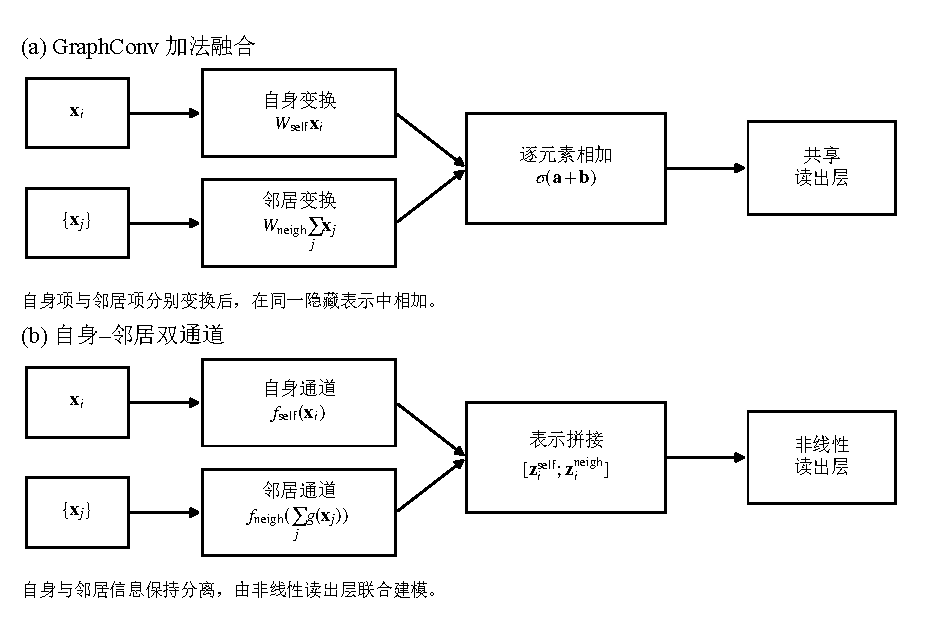
\includegraphics[width=\textwidth]{architecture_compare.pdf}
  \caption{融合式 GraphConv 基线与自身--邻居双通道模型。
(a) 基线对自身项和邻居项分别变换后相加；
(b) 双通道将自身演化与邻居交互保持到读出阶段，
从而缓解量级失衡和表示混合。}
  \label{fig:architecture}
\end{figure}

\subsection{对照模型与评价设计}

为理解表示选择带来的影响，已知网络实验比较五个模型：单向求和 GraphConv、双向求和 GraphConv、增加隐藏非线性的双向求和 GraphConv、双向均值 GraphConv以及双向双通道模型。
这里的“单向”并非一种合理的无向网络模型，
而是边表未显式补齐反向消息时的实现缺陷对照；
它用于说明网络数据进入消息传递框架时，
边方向处理同样会影响所学规律。

比较并不只看一步分类结果。
感染概率随邻居数变化的曲线用于判断模型是否学到了正确的交互响应，参数反演用于概括曲线与真实机制的接近程度，
多步自回归则检验小的一步偏差是否会在闭环中累积。
这样的多层评价能够区分两类模型：一种只是对当前样本分类较准，
另一种同时保留了可解释且可推演的动力学关系。
具体层数、训练轮数和优化参数列于附录。
